\documentclass[11pt,a4paper]{article}
\usepackage[a4paper,margin=2.4cm]{geometry}
\usepackage[T1]{fontenc}
\usepackage{lmodern}
\usepackage{microtype}
\usepackage{amsmath,amssymb,mathtools,amsthm}
\usepackage{booktabs,array,tabularx}
\usepackage{enumitem}
\usepackage[most]{tcolorbox}
\usepackage{tikz}
\usetikzlibrary{arrows.meta,positioning,calc,decorations.pathreplacing}
\usepackage{caption}
\usepackage{float}
\usepackage{fancyhdr}
\usepackage{xcolor}
\usepackage[hidelinks]{hyperref}

\definecolor{mblue}{HTML}{1F4E79}
\definecolor{mgrey}{HTML}{F4F6F9}
\definecolor{morange}{HTML}{B5591F}

\newtcolorbox{modelbox}[1]{enhanced,breakable,colback=mgrey,colframe=mblue,
  boxrule=0.8pt,arc=2pt,left=6pt,right=6pt,top=4pt,bottom=4pt,
  title={#1},fonttitle=\bfseries\small,coltitle=white}
\newtcolorbox{notebox}[1][Remark]{enhanced,breakable,colback=white,colframe=morange,
  boxrule=0.6pt,arc=2pt,left=6pt,right=6pt,top=3pt,bottom=3pt,
  title={#1},fonttitle=\bfseries\small,coltitle=white}

\newtheorem{lemma}{Lemma}
\theoremstyle{definition}
\newtheorem{assumption}{Assumption}

\setlist{itemsep=2pt,topsep=3pt}
\setlength{\parindent}{0pt}
\setlength{\parskip}{5pt}
\pagestyle{fancy}
\fancyhf{}
\fancyhead[L]{\small ME44207 Group Assignment Q2 -- Mathematical models}
\fancyhead[R]{\small Group \textless nr\textgreater}
\fancyfoot[C]{\small\thepage}
\renewcommand{\headrulewidth}{0.4pt}

\newcommand{\R}{\mathbb{R}}
\newcommand{\Z}{\mathbb{Z}}
\newcommand{\dout}{\delta^{+}}
\newcommand{\din}{\delta^{-}}
\newcommand{\sumk}{\sum_{k\in K}}
\newcommand{\sumA}{\sum_{(i,j)\in A}}

\begin{document}

\begin{titlepage}
\centering
\vspace*{3cm}
{\large ME44207 Quantitative Methods for Logistics\par}
\vspace{4pt}
{\large Group Assignment Q2 -- 2026\par}
\vspace{1.4cm}
{\LARGE\bfseries Electric Vehicle Routing with Time Windows\\[4pt] and an Uncertain Driving Range\par}
\vspace{0.8cm}
{\Large Mathematical models, derivations and explanation\par}
\vspace{2.2cm}
\begin{tabular}{rl}
Group number: & \textless\ group number \textgreater\\
Members: & \textless\ name 1 \textgreater, \textless\ name 2 \textgreater, \textless\ name 3 \textgreater, \textless\ name 4 \textgreater
\end{tabular}
\vfill
{\small This document belongs to the Python/Gurobi files \texttt{vrp\_common.py}, \texttt{part1\_deterministic.py}, \texttt{part2\_chance\_constrained.py}, \texttt{part3\_recourse.py} and \texttt{part3d\_depot\_recharging.py}.\par}
\end{titlepage}

{\small\tableofcontents}
\newpage

%==========================================================================================
\section{Introduction and reading guide}
%==========================================================================================
A fleet of identical electric vehicles collects at a set of pickup locations, starting and ending at one depot. Every location has to be visited exactly once within its time window, and every visit takes a fixed service time. The complication is the \emph{driving range} of the vehicles: it depends on the month (battery performance is lower in winter) and is therefore uncertain when the routes are planned. The assignment treats this uncertainty in three increasingly rich ways, which leads to the family of models in this document.

\begin{figure}[H]
\centering
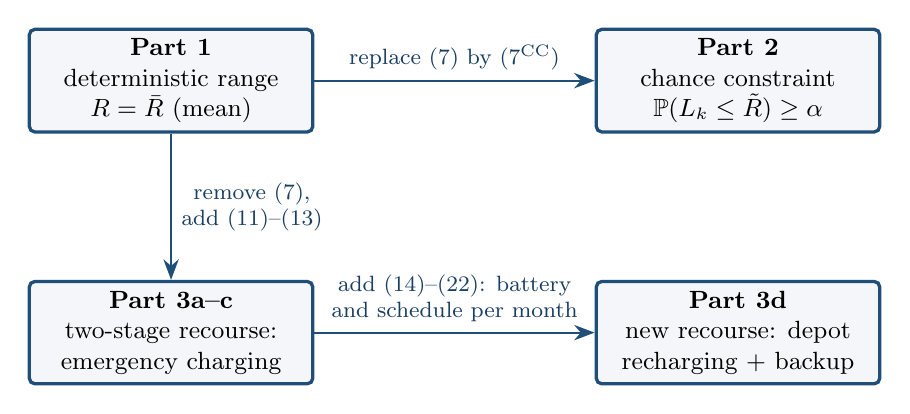
\begin{tikzpicture}[
  box/.style={draw=mblue,very thick,rounded corners=2pt,fill=mgrey,align=center,minimum width=3.6cm,minimum height=1.3cm,font=\small},
  arr/.style={-{Stealth[length=2.6mm]},thick,mblue},
  lab/.style={font=\footnotesize,align=center,text=mblue!80!black}]
\node[box] (p1) at (0,0) {\textbf{Part 1}\\ deterministic range\\ $R=\bar R$ (mean)};
\node[box] (p2) at (7.2,0) {\textbf{Part 2}\\ chance constraint\\ $\mathbb P(L_k\le\tilde R)\ge\alpha$};
\node[box] (p3) at (0,-3.2) {\textbf{Part 3a--c}\\ two-stage recourse:\\ emergency charging};
\node[box] (p4) at (7.2,-3.2) {\textbf{Part 3d}\\ new recourse: depot\\ recharging + backup};
\draw[arr] (p1) -- node[lab,above]{replace (7) by (7$^{\mathrm{CC}}$)} (p2);
\draw[arr] (p1) -- node[lab,right]{remove (7),\\ add (11)--(13)} (p3);
\draw[arr] (p3) -- node[lab,above]{add (14)--(22): battery\\ and schedule per month} (p4);
\end{tikzpicture}
\caption{How the models build on each other. The routing core (constraints (1)--(6) and (8)--(10)) is shared by all models; only the way the range is handled changes.}
\label{fig:hierarchy}
\end{figure}

\textbf{Structure of every chapter.} Each model is first given compactly in a blue box (this is the form to use in the report). It is followed by (i) an explanation of the objective and of every constraint, (ii) the derivations needed (big-$M$ values, deterministic equivalent, number of recharges), and (iii) remarks on modelling choices and implementation. Orange boxes contain remarks that are useful for the discussion part of the report.

\textbf{General conventions.}
\begin{itemize}
\item Distances are Euclidean. One distance unit is also one time unit (minutes) and one cost unit. Hence $d_{ij}$ is at the same time the distance, the travel time and the travel cost of arc $(i,j)$.
\item The data files are read as they are. The end depot $n+1$ (a copy of the depot) is created in Python after reading; it is not added to the file.
\item Equation numbers are the same as in \texttt{SOLUTION\_NOTES.md} and in the comments of the code.
\end{itemize}

\begin{table}[H]
\centering\small
\begin{tabularx}{\textwidth}{@{}l X l l@{}}
\toprule
Part & How the range is treated & Range constraints & Objective\\
\midrule
1 & deterministic, $R=\bar R=119.28$ & (7) & distance\\
2 & random $\tilde R\sim N(\mu,\sigma^2)$, chance constraint & (7$^{\mathrm{CC}}$) $\Leftrightarrow$ (7$'$) & distance\\
3a--c & 12 monthly scenarios, recourse = emergency charging & (11)--(13) & distance + E[penalty]\\
3d & 12 scenarios, recourse = depot recharging or emergency & (14)--(22) & distance + E[recourse]\\
\bottomrule
\end{tabularx}
\caption{Overview of the models.}
\end{table}

%==========================================================================================
\section{Common notation}
%==========================================================================================
\begin{table}[H]
\centering\small
\renewcommand{\arraystretch}{1.15}
\begin{tabularx}{\textwidth}{@{}l X@{}}
\toprule
\multicolumn{2}{@{}l}{\textbf{Sets}}\\
$N=\{0,1,\dots,n\}$ & locations as in the data file; $0$ is the depot \\
$C=N\setminus\{0\}$ & pickup locations (customers) \\
$V=N\cup\{n+1\}$ & all nodes; $n+1$ is a copy of the depot that marks the end of a route \\
$A$ & arcs: $\{(0,j):j\in C\cup\{n+1\}\}\cup\{(i,j):i\in C,\ j\in C\cup\{n+1\},\ i\neq j\}$ \\
$\dout(i),\ \din(j)$ & successors $\{j:(i,j)\in A\}$ and predecessors $\{i:(i,j)\in A\}$ \\
$K=\{1,\dots,m\}$ & vehicles (identical) \\
\midrule
\multicolumn{2}{@{}l}{\textbf{Parameters}}\\
$d_{ij}$ & Euclidean distance = travel time = travel cost of arc $(i,j)$; $d_{0,n+1}=0$ \\
$[e_i,l_i]$ & time window (ready time, due time); $e_{n+1}=e_0$, $l_{n+1}=l_0$ \\
$s_i$ & service time; $s_0=s_{n+1}=0$ \\
$R$ & driving range of a vehicle (Part 1: $R=\bar R$, the mean of the 12 monthly ranges) \\
$M^D_{ij},\ M^T_{ij}$ & big-$M$ constants (Section~\ref{sec:bigm}) \\
\midrule
\multicolumn{2}{@{}l}{\textbf{Decision variables}}\\
$x_{ijk}\in\{0,1\}$ & $=1$ if vehicle $k$ drives from $i$ to $j$ \\
$T_{ik}\ge 0$ & time at which vehicle $k$ starts service at node $i$ \\
$D_{ik}\ge 0$ & distance driven by vehicle $k$ when it arrives at node $i$ \\
\bottomrule
\end{tabularx}
\caption{Notation used in all models.}
\label{tab:notation}
\end{table}

\textbf{Derived quantities.} The length of the route of vehicle $k$ is $L_k=\sum_{(i,j)\in A}d_{ij}x_{ijk}$. The remaining range of vehicle $k$ on arrival at node $i$ is $r_{ik}=R-D_{ik}$. A vehicle is used if it does not take the ``empty'' arc $(0,n+1)$: $u_k=1-x_{0,n+1,k}$.

\begin{figure}[H]
\centering
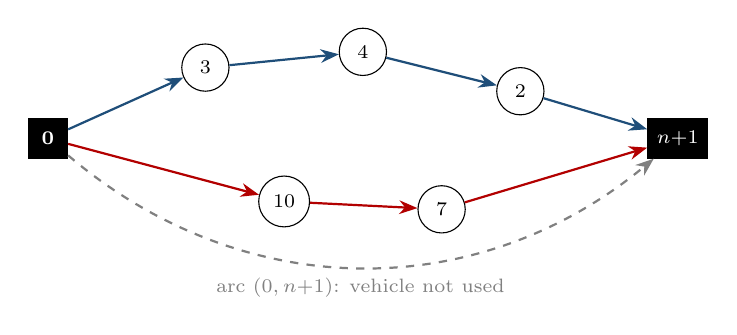
\begin{tikzpicture}[>=Stealth,
  dep/.style={draw,fill=black,minimum size=5mm,text=white,font=\scriptsize\bfseries},
  cus/.style={draw,circle,minimum size=6mm,font=\scriptsize}]
\node[dep] (s) at (0,0) {0};
\node[cus] (a) at (2,0.9) {3};
\node[cus] (b) at (4,1.1) {4};
\node[cus] (c) at (6,0.6) {2};
\node[dep] (e) at (8,0) {$n{+}1$};
\node[cus] (f) at (3,-0.8) {10};
\node[cus] (g) at (5,-0.9) {7};
\draw[->,thick,mblue] (s)--(a); \draw[->,thick,mblue] (a)--(b); \draw[->,thick,mblue] (b)--(c); \draw[->,thick,mblue] (c)--(e);
\draw[->,thick,red!70!black] (s)--(f); \draw[->,thick,red!70!black] (f)--(g); \draw[->,thick,red!70!black] (g)--(e);
\draw[->,thick,dashed,gray] (s) to[bend right=40] node[below,font=\scriptsize]{arc $(0,n{+}1)$: vehicle not used} (e);
\end{tikzpicture}
\caption{Every vehicle is a path from node $0$ to node $n+1$ (same location). An unused vehicle takes the zero-length arc $(0,n+1)$.}
\end{figure}

%==========================================================================================
\section{Part 1a -- Deterministic model}
%==========================================================================================
\subsection{Assumptions}
\begin{itemize}
\item Every vehicle has the same range $R=\bar R=\frac1{12}\sum_{t=1}^{12}R_t=119.28$, the mean of the monthly ranges.
\item Every vehicle starts and ends at the depot. It may wait at a location if it arrives before the ready time; service must \emph{start} no later than the due time.
\item The range is consumed only by driving (service and waiting do not use range). There is no charging during the day.
\item The objective is the total distance driven. There is no fixed cost per vehicle, so unused vehicles cost nothing.
\end{itemize}

\subsection{Model}
\begin{modelbox}{Model P1: deterministic VRP with time windows and range}
\begin{align*}
\min\quad & \sumk\sumA d_{ij}\,x_{ijk} \tag{0}\\[3pt]
\text{s.t.}\quad
& \sumk\sum_{j\in\dout(i)} x_{ijk}=1 && \forall i\in C \tag{1}\\
& \sum_{j\in\dout(0)} x_{0jk}=1 && \forall k\in K \tag{2}\\
& \sum_{i\in\din(h)} x_{ihk}-\sum_{j\in\dout(h)} x_{hjk}=0 && \forall h\in C,\ k\in K \tag{3}\\
& \sum_{i\in\din(n+1)} x_{i,n+1,k}=1 && \forall k\in K \tag{4}\\
& D_{0k}=0 && \forall k\in K \tag{5}\\
& D_{jk}\ \ge\ D_{ik}+d_{ij}-M^D_{ij}\,(1-x_{ijk}) && \forall (i,j)\in A,\ k\in K \tag{6}\\
& D_{n+1,k}\ \le\ R && \forall k\in K \tag{7}\\
& T_{jk}\ \ge\ T_{ik}+s_i+d_{ij}-M^T_{ij}\,(1-x_{ijk}) && \forall (i,j)\in A,\ k\in K \tag{8}\\
& e_i\ \le\ T_{ik}\ \le\ l_i && \forall i\in V,\ k\in K \tag{9}\\
& x_{ijk}\in\{0,1\},\quad D_{ik}\ge0,\quad T_{ik}\ge0 && \forall (i,j)\in A,\ i\in V,\ k\in K \tag{10}
\end{align*}
\textbf{Without time windows:} drop (8)--(9) (and the variables $T_{ik}$).
\end{modelbox}

\subsection{Explanation of the objective and the constraints}
\begin{description}[leftmargin=1.1cm,style=sameline,font=\normalfont\bfseries]
\item[(0)] Total distance driven by all vehicles. Since distance, time and cost are measured in the same unit, this is also the total driving time and cost.
\item[(1)] Every pickup location is left exactly once, by exactly one vehicle. Together with flow conservation (3) it is therefore also entered exactly once: every location is visited exactly once.
\item[(2)] Every vehicle leaves the depot exactly once. Because the arc $(0,n+1)$ is part of $A$, a vehicle that is not needed takes this ``empty'' arc. This makes the model valid for any number of vehicles $m$: the model itself decides how many are used.
\item[(3)] Flow conservation: a vehicle that enters location $h$ also leaves it. This makes sure that the arcs of one vehicle form one connected path.
\item[(4)] Every vehicle ends its route exactly once at the end depot $n+1$.
\item[(5)] The ``odometer'' of every vehicle is $0$ when it leaves the depot.
\item[(6)] Distance accumulation: if vehicle $k$ drives arc $(i,j)$, then the distance driven on arrival at $j$ is at least that on arrival at $i$ plus $d_{ij}$. If the arc is not used, the big-$M$ term makes the constraint redundant. At the end depot, $D_{n+1,k}$ is therefore at least the route length $L_k$. Constraint (6) also eliminates subtours (Section~\ref{sec:subtour}).
\item[(7)] Range constraint: the total distance of each vehicle may not exceed its range. Since $D_{n+1,k}\ge L_k$, this guarantees $L_k\le R$.
\item[(8)] Time propagation: if vehicle $k$ drives arc $(i,j)$, service at $j$ can start only after service at $i$ is finished and the vehicle has driven to $j$. Waiting is allowed ($\ge$ instead of $=$).
\item[(9)] Service must start within the time window. For the end depot it means the vehicle is back before the depot closes ($l_{n+1}=l_0$).
\item[(10)] Domains of the variables.
\end{description}

\subsection{Big-$M$ values}\label{sec:bigm}
A big-$M$ must be large enough to make the constraint redundant when $x_{ijk}=0$, but as small as possible to keep the LP relaxation tight.
\begin{itemize}
\item \textbf{Time.} For $x_{ijk}=0$, constraint (8) must hold for all values allowed by (9). The worst case is $T_{ik}=l_i$ and $T_{jk}=e_j$, which requires $e_j\ge l_i+s_i+d_{ij}-M^T_{ij}$, so
\[ M^T_{ij}=\max\{0,\ l_i+s_i+d_{ij}-e_j\}. \]
\item \textbf{Distance.} With bounds $\underline D_i\le D_{ik}\le\overline D_i$, the worst case is $D_{ik}=\overline D_i$, $D_{jk}=\underline D_j$, so
\[ M^D_{ij}=\max\{0,\ \overline D_i+d_{ij}-\underline D_j\}. \]
With the simple bounds $0\le D_{ik}\le R$ this gives $M^D_{ij}=R+d_{ij}$. The code uses the tighter bounds of Section~\ref{sec:impl}.
\end{itemize}

\subsection{Why (6) and (8) eliminate subtours}\label{sec:subtour}
Suppose vehicle $k$ uses a cycle of customers $i_1\to i_2\to\dots\to i_p\to i_1$ that is not connected to the depot. For all arcs on the cycle $x=1$, so (6) gives $D_{i_2k}\ge D_{i_1k}+d_{i_1i_2}$, \dots, $D_{i_1k}\ge D_{i_pk}+d_{i_pi_1}$. Adding these inequalities gives
\[ 0\ \ge\ \textstyle\sum_{\text{arcs on the cycle}} d_{ij} \;>\;0, \]
a contradiction, because all locations have different coordinates, so $d_{ij}>0$. In the same way (8) eliminates subtours, since $s_i+d_{ij}>0$. Hence no separate subtour-elimination constraints are needed. This is the same idea as the MTZ constraints of the TSP, with distance (or time) taking the role of the order variable $u_i$.

\subsection{Variant without time windows}
Without time windows, constraints (8)--(9) are removed. Constraint (6) then does both jobs: it measures the route length for the range constraint, and it eliminates subtours. The times of visit are then computed afterwards from the routes: the vehicle leaves at $t=0$ and service starts on arrival.

\subsection{Implementation enhancements (do not change the optimum)}\label{sec:impl}
The following additions are valid for every feasible solution, so they do not change the optimal value. They only make the model smaller or the LP relaxation tighter.
\begin{enumerate}
\item \textbf{Arc pre-processing (only with time windows).} An arc $(i,j)$ with $e_i+s_i+d_{ij}>l_j$ can never be used: even the earliest possible service at $i$ reaches $j$ too late. Such arcs are removed from $A$. For the small instance this reduces $|A|$ from 111 to 72.
\item \textbf{Tighter bounds on $D$.} A vehicle that arrives at customer $i$ has driven at least $d_{0i}$, and still has to drive back at least $d_{i0}$:
\[ d_{0i}\ \le\ D_{ik}\ \le\ R-d_{i0}\qquad\forall i\in C,\ k\in K. \]
These bounds are used for $\underline D_i,\overline D_i$ in $M^D_{ij}$.
\item \textbf{Symmetry breaking.} The vehicles are identical, so every solution exists $m!$ times with the vehicle numbers permuted. Ordering the vehicles by route length removes these copies:
\[ \sumA d_{ij}x_{ijk}\ \ge\ \sumA d_{ij}x_{ij,k+1}\qquad k=1,\dots,m-1. \tag{SB}\]
It also implies that vehicle $k+1$ is only used if vehicle $k$ is used.
\end{enumerate}
\begin{notebox}[Effect of the enhancements]
In the no-time-window case the enhancements reduced the solve time by roughly a factor 10 in our tests. The optimal objective values did not change, as expected. Without time windows the problem is harder because only the weak constraints (6) remove subtours and many more arcs are possible.
\end{notebox}

\subsection{Reported output}
For every vehicle the route, its length and the remaining range at the end ($R-L_k$) are reported. For every node, the time of visit and the remaining range on arrival ($R-D_{ik}$) are reported. Because (6) and (8) are inequalities, the solver values of $D$ and $T$ may contain slack. The code therefore recomputes them along each route: the vehicle leaves the depot just in time for its first pickup, service starts at $\max(\text{arrival},e_j)$, and the remaining range is $R$ minus the distance driven so far. This recomputation is also used as an independent feasibility check.

%==========================================================================================
\section{Part 2a -- Chance-constrained model}
%==========================================================================================
\subsection{Range distribution}
The range is now a random variable $\tilde R\sim N(\mu,\sigma^2)$. Both parameters are estimated from the 12 monthly ranges $R_1,\dots,R_{12}$:
\[
\hat\mu=\frac1{12}\sum_{t=1}^{12}R_t=119.28,\qquad
\hat\sigma=\sqrt{\frac1{11}\sum_{t=1}^{12}(R_t-\hat\mu)^2}=17.28 .
\]
The sample standard deviation (divisor $n-1=11$) is the unbiased estimator; with only 12 observations the difference with the population formula ($\hat\sigma=16.54$) is not negligible, and the sample version is the more conservative one.

\subsection{Chance constraint}
The deterministic range constraint (7) is replaced by the requirement that every vehicle can complete its route with probability at least $\alpha$:
\begin{modelbox}{Chance constraint (individual, per vehicle)}
\[
\mathbb P\big(D_{n+1,k}\le\tilde R\big)\ \ge\ \alpha\qquad\forall k\in K \tag{7$^{\mathrm{CC}}$}
\]
equivalently $\mathbb P\big(D_{n+1,k}>\tilde R\big)\le 1-\alpha$: the probability that a vehicle runs out of range is at most $1-\alpha$.
\end{modelbox}

\subsection{Derivation of the deterministic equivalent}
For given routes, $D_{n+1,k}$ is a deterministic number $D$. Only the right-hand side is random. Standardise with $Z=(\tilde R-\mu)/\sigma\sim N(0,1)$ and let $\Phi$ be its distribution function:
\begin{align*}
\mathbb P(\tilde R\ge D)\ge\alpha
&\iff \mathbb P\Big(Z\ge \tfrac{D-\mu}{\sigma}\Big)\ge\alpha
\iff 1-\Phi\Big(\tfrac{D-\mu}{\sigma}\Big)\ge\alpha
\iff \Phi\Big(\tfrac{D-\mu}{\sigma}\Big)\le 1-\alpha\\
&\iff \tfrac{D-\mu}{\sigma}\le \Phi^{-1}(1-\alpha)=-\Phi^{-1}(\alpha)=-z_\alpha
\iff D\le \mu-z_\alpha\,\sigma .
\end{align*}
Hence (7$^{\mathrm{CC}}$) is \emph{exactly} equivalent to the linear constraint
\begin{modelbox}{Deterministic equivalent}
\[
D_{n+1,k}\ \le\ R_\alpha:=\mu-z_\alpha\,\sigma\qquad\forall k\in K,\qquad z_\alpha=\Phi^{-1}(\alpha). \tag{7$'$}
\]
\end{modelbox}
This is not an approximation. The reformulation is exact because the uncertainty is only in the right-hand side and its distribution is fully known. The model therefore stays a MILP of the same size as P1.

\begin{table}[H]
\centering\small
\begin{tabular}{@{}cccc@{}}
\toprule
$\alpha$ & $z_\alpha$ & $R_\alpha=\mu-z_\alpha\sigma$ & months with $R_t<R_\alpha$\\
\midrule
0.50 & 0.0000 & 119.28 & 5 \\
0.75 & 0.6745 & 107.63 & 3 \\
0.90 & 1.2816 & 97.14 & 2 \\
0.99 & 2.3263 & 79.09 & 0 \\
\bottomrule
\end{tabular}
\caption{Right-hand side of (7$'$) for the tested confidence levels.}
\end{table}

\subsection{Complete chance-constrained model}
\begin{modelbox}{Model P2: chance-constrained VRP(TW)}
\[
\min\ (0)\quad\text{s.t. } (1)\text{--}(6),\ (7'),\ (8)\text{--}(10),\qquad M^D_{ij}\text{ computed with } R_\alpha \text{ instead of } R.
\]
Compared with P1, only the parameter $R$ in (7) and in the bounds/big-$M$ of $D$ is replaced by $R_\alpha$. New parameters: $\alpha$, $\mu$, $\sigma$, $z_\alpha$, $R_\alpha$. No new variables.
\end{modelbox}

\subsection{Individual versus joint chance constraint}
A joint chance constraint would require that \emph{all} vehicles can finish their routes simultaneously with probability $\alpha$:
\[
\mathbb P\big(D_{n+1,k}\le\tilde R\ \ \forall k\in K\big)\ge\alpha .
\]
In this problem every vehicle faces the \emph{same} range on a given day (one random variable $\tilde R$). The event ``all vehicles can finish'' equals ``the longest route can finish'', so
\[
\mathbb P\big(\max_k D_{n+1,k}\le\tilde R\big)\ge\alpha\iff \max_k D_{n+1,k}\le R_\alpha\iff D_{n+1,k}\le R_\alpha\ \ \forall k .
\]
The joint and the individual chance constraint therefore lead to exactly the same model. This would not be true if the vehicles had independent ranges.

\begin{notebox}[Remarks for the discussion]
\begin{itemize}
\item $\alpha=0.5$ gives $z_\alpha=0$ and $R_\alpha=\mu$: model P2 is then identical to P1. The deterministic model with the mean range only guarantees a 50\% probability that a route can be completed.
\item Increasing $\alpha$ lowers the distance budget $R_\alpha$. The cost rises in steps: the solution only changes once the current routes no longer fit. With 3 vehicles, $\alpha=0.99$ ($R_\alpha=79.09$) is infeasible.
\item The 12 monthly ranges show a clear seasonal pattern (low in winter, high in summer) and are not really normally distributed. For $\alpha=0.99$ the normal model gives $R_\alpha=79.09$, below the lowest range ever observed (89.35): the normal tail is very conservative here. A check of each solution against the 12 real months shows how often a route would actually fail.
\item A chance constraint limits \emph{how often} the range is exceeded, but not \emph{how costly} an exceedance is. Part 3 adds exactly that.
\end{itemize}
\end{notebox}

%==========================================================================================
\section{Part 3a -- Two-stage stochastic model with recourse}
%==========================================================================================
\subsection{Scenarios and stages}
The range distribution is now represented by the 12 observed months, each an equally likely scenario.
\begin{itemize}
\item $S=\{1,\dots,12\}$: scenarios (months), with probability $p_s=1/12$ and range $R_s$.
\item $P$: penalty (cost) of one emergency recharge, in distance units.
\end{itemize}
\textbf{First stage} (here and now, before the range is known): the routes $x_{ijk}$, together with $D_{ik}$ and the nominal schedule $T_{ik}$. One plan is used for the whole year.\\
\textbf{Second stage} (wait and see, once the month and so $R_s$ is known): the number of emergency recharges $n_{ks}\in\Z_{\ge0}$ of vehicle $k$ in scenario $s$.

\subsection{Number of recharges as a function of the route length}
\begin{assumption}
Emergency charging is possible anywhere along the route, restores the range to $R_s$, takes no time, causes no detour and costs $P$ per charge.
\end{assumption}

\begin{lemma}\label{lem:ceil}
A route of length $L>0$ driven with range $R_s$ needs exactly $\max\{0,\lceil L/R_s\rceil-1\}$ emergency recharges.
\end{lemma}
\begin{proof}
With $n$ recharges the vehicle can drive at most $(n+1)R_s$ (the initial battery plus $n$ full charges), so $n\ge L/R_s-1$. Since $n$ is integer, $n\ge\lceil L/R_s\rceil-1$. Charging exactly when the battery is empty achieves this number.
\end{proof}

\begin{figure}[H]
\centering
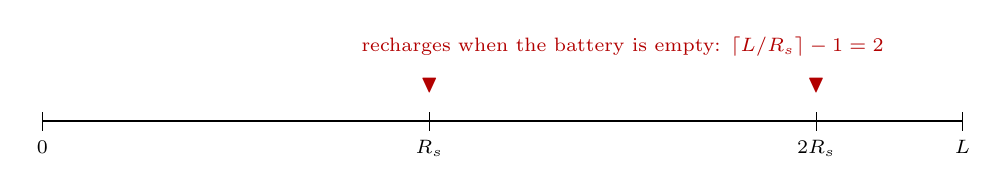
\begin{tikzpicture}[x=0.055cm]
\draw[thick] (0,0)--(212.5,0);
\foreach \p/\l in {0/0, 89.35/{$R_s$}, 178.7/{$2R_s$}} {\draw (\p,-0.12)--(\p,0.12); \node[below,font=\scriptsize] at (\p,-0.12) {\l};}
\draw (212.5,-0.12)--(212.5,0.12); \node[below,font=\scriptsize] at (212.5,-0.12) {$L$};
\foreach \p in {89.35,178.7} {\node[red!70!black] at (\p,0.45) {\small$\blacktriangledown$};}
\node[font=\scriptsize,red!70!black,align=center] at (134,0.95) {recharges when the battery is empty: $\lceil L/R_s\rceil-1=2$};
\end{tikzpicture}
\caption{Lemma~\ref{lem:ceil}: a route of length $L$ between $2R_s$ and $3R_s$ needs two recharges.}
\end{figure}

The non-linear ceiling function is linearised with the integer variable $n_{ks}$:
\[
R_s\,(1+n_{ks})\ \ge\ L_k,\qquad n_{ks}\in\Z_{\ge 0}.
\]
Because $n_{ks}$ has a positive cost in a minimisation problem, it will take the smallest integer value that satisfies the constraint, which is exactly $\lceil L_k/R_s\rceil-1$ (or $0$).

\subsection{Model}
\begin{modelbox}{Model P3: two-stage stochastic VRP(TW) with emergency charging (extensive form)}
\begin{align*}
\min\quad & \sumk\sumA d_{ij}\,x_{ijk}\;+\;\sum_{s\in S}p_s\sumk P\,n_{ks} \tag{0$'$}\\[3pt]
\text{s.t.}\quad
& (1)\text{--}(6),\ (8)\text{--}(10)\quad\text{(range constraint (7) removed; } D_{ik}\le U)\\
& R_s\,(u_k+n_{ks})\ \ge\ \sumA d_{ij}\,x_{ijk} && \forall k\in K,\ s\in S \tag{11}\\
& u_k = 1-x_{0,n+1,k} && \forall k\in K \tag{12}\\
& n_{ks}\in\{0,1,\dots,n^{\max}\} && \forall k\in K,\ s\in S \tag{13}
\end{align*}
with $U=\sum_{i\in\{0\}\cup C}\max_{j\in\dout(i)}d_{ij}$ (upper bound on any route length) and $n^{\max}=\lceil U/\min_s R_s\rceil$.
\end{modelbox}

\subsection{Explanation}
\begin{description}[leftmargin=1.1cm,style=sameline,font=\normalfont\bfseries]
\item[(0$'$)] First-stage cost (distance, the same every day) plus the \emph{expected} second-stage cost: the penalty $P$ times the expected number of recharges per day. With $p_s=1/12$ this equals $\frac{P}{12}\times$ the total number of recharges over the 12 months. Minimising the expected cost is therefore the same as trading off distance against the total number of recharges over all scenarios.
\item[(1)--(6), (8)--(10)] Routing core as in P1. The range is no longer a hard constraint (a vehicle may exceed it, at a cost). $D_{ik}$ now only measures distance and eliminates subtours, so its upper bound becomes $U$ instead of $R$ (and $M^D_{ij}$ accordingly).
\item[(11)] Lemma~\ref{lem:ceil} in linear form: the range in scenario $s$ times the number of ``battery fills'' (the first one plus $n_{ks}$ recharges) must cover the route length $L_k$.
\item[(12)] $u_k=1$ if vehicle $k$ is used. Using $u_k$ instead of the constant 1 in (11) is equivalent for integer solutions: an unused vehicle has $L_k=0$ and needs $n_{ks}=0$. In the LP relaxation, however, $u_k$ can be fractional, which makes (11) tighter and speeds up the solver considerably.
\item[(13)] Number of recharges, integer and bounded.
\end{description}

\subsection{Two-stage interpretation}
In compact form the model is
\begin{align*}
&\min_{x\in X}\ \Big\{\,d^\top x+\mathbb E_s\big[Q(x,s)\big]\Big\},\qquad\text{with}\\
&Q(x,s)=\min_{n\in\Z^{m}_{\ge0}}\Big\{P\sumk n_{k}\ :\ R_s(u_k+n_k)\ge L_k(x)\ \forall k\Big\}=P\sumk\Big(\Big\lceil\tfrac{L_k(x)}{R_s}\Big\rceil-1\Big)^{+},
\end{align*}
where $X$ is the set of routes satisfying (1)--(6), (8)--(10). Because there are only 12 scenarios, the expectation is written out in full (extensive form / deterministic equivalent) and solved as one MILP. The second stage always has a feasible solution, whatever the routes (\emph{complete recourse}): any route can be completed with enough recharges.

\begin{notebox}[Useful concepts for the discussion]
\begin{itemize}
\item \textbf{EV problem.} Model P1 is exactly the \emph{expected value problem}: the random range is replaced by its mean.
\item \textbf{EEV.} The expected cost of the P1 solution evaluated in model P3: its distance plus $\frac{P}{12}\times$ the recharges it needs in the 12 months.
\item \textbf{RP.} The optimal value of P3 (recourse problem).
\item \textbf{VSS} $=\text{EEV}-\text{RP}\ge0$: the value of the stochastic solution, i.e.\ what is saved by taking the range distribution into account instead of planning with the mean.
\item The penalty $P$ determines the trade-off. Low $P$: drive the shortest plan and accept recharges. High $P$: use more vehicles and more distance so that no route exceeds the range of the worst month.
\end{itemize}
\end{notebox}

\textbf{Parts 3b and 3c} use this same model; only the data change: the small instance with $m=3$ (with and without time windows) for 3b, and the large instance (21 locations) with time windows and $m=5$ for 3c. For 3c, $m=5$ is the smallest fleet for which a plan without any recharge exists (all routes $\le\min_sR_s=89.35$), which mirrors the role of $m=3$ for the small instance.

%==========================================================================================
\section{Part 3d -- New recourse: depot recharging during idle time}
%==========================================================================================
\subsection{Motivation}
The results of Part 1 show long idle periods caused by the time windows (up to about 600 minutes of waiting at a location). In practice an operator of an electric fleet would rather use such idle time to recharge at its own depot than call expensive emergency charging. The new recourse strategy therefore lets a vehicle, in a month with a low range, \emph{detour via the depot} between two consecutive pickups ($i\to0\to j$ instead of $i\to j$) and fast-charge there. Unlike emergency charging in 3b, this detour costs \emph{time}. It is only possible if all later time windows can still be met in that month, so the schedule becomes scenario-dependent. Emergency charging remains available as a backup.

\subsection{Assumptions}
\begin{itemize}
\item A depot recharge restores the full range $R_s$ in a fixed time $\tau$ (fast charger), and costs the extra distance $d_{i0}+d_{0j}-d_{ij}$ plus a fixed handling cost $F$.
\item A detour is only made between two pickups. Before the first pickup the battery is full, and after the last pickup the vehicle drives to the depot anyway.
\item A vehicle must reach the depot on its own battery; at most one recourse action is taken per arc.
\item Emergency charging is as in 3b (penalty $P$, no time, no detour).
\item The routes (first stage) are the same in every month; battery levels, detours, emergency charges and the timetable may differ per month (second stage).
\end{itemize}

\subsection{Additional notation}
\begin{table}[H]
\centering\small
\renewcommand{\arraystretch}{1.15}
\begin{tabularx}{\textwidth}{@{}l X@{}}
\toprule
$\tau$, $F$ & depot charging time ($\tau=30$) and fixed cost per depot recharge ($F=5$)\\
$A^Z$ & arcs on which a detour can fit in time: $\{(i,j)\in A:\ i,j\in C,\ e_i+s_i+d_{i0}+\tau+d_{0j}\le l_j\}$\\
$A^W$ & arcs on which emergency charging is possible: $A\setminus\{(0,n+1)\}$\\
$y_{ij}$ & $=\sumk x_{ijk}$, $=1$ if arc $(i,j)$ is used by any vehicle (an expression, not a new variable)\\
\midrule
$z_{ijs}\in\{0,1\}$ & $=1$ if in month $s$ the vehicle on arc $(i,j)$ detours via the depot to recharge\\
$w_{ijs}\in\{0,1\}$ & $=1$ if in month $s$ an emergency recharge takes place on arc $(i,j)$\\
$b_{is}\in[0,R_s]$ & remaining range on arrival at location $i\in C$ in month $s$\\
$T^s_i\in[e_i,l_i]$ & start of service at location $i\in C$ in month $s$\\
\bottomrule
\end{tabularx}
\caption{Additional notation for Part 3d. For $(i,j)\notin A^Z$ we set $z_{ijs}:=0$.}
\end{table}
Every location is visited by exactly one vehicle, and every arc between locations is used by at most one vehicle. Therefore the second-stage variables need no vehicle index: they are linked to the routes through $y_{ij}$.

\subsection{Model}
\begin{modelbox}{Model P3d: two-stage VRPTW with depot recharging and emergency backup}
\vspace{-6pt}
\begin{align*}
\min\quad & \sumk\sumA d_{ij}x_{ijk}+\sum_{s\in S}p_s\Big[\sum_{(i,j)\in A^Z}\big(F+d_{i0}+d_{0j}-d_{ij}\big)z_{ijs}+\sum_{(i,j)\in A^W}P\,w_{ijs}\Big] \tag{0$''$}
\end{align*}
\vspace{-4pt}
subject to (1)--(6), (8)--(10) (first stage, $D_{ik}\le U$) and for all $s\in S$:
\begin{align*}
& z_{ijs}+w_{ijs}\le y_{ij} && (i,j)\in A^W \tag{14}\\
& b_{js}\le R_s-d_{0j}+R_s\,w_{0js}+d_{0j}\,(1-y_{0j}) && j\in C \tag{15}\\
& b_{js}\le b_{is}-d_{ij}+R_s\,w_{ijs}+(R_s+d_{ij})(1-y_{ij}+z_{ijs}) && (i,j)\in A,\ i,j\in C \tag{16}\\
& b_{is}\ge d_{i0}\,z_{ijs},\qquad b_{js}\le R_s-d_{0j}+d_{0j}\,(1-z_{ijs}) && (i,j)\in A^Z \tag{17}\\
& b_{is}+R_s\,w_{i,n+1,s}\ge d_{i0}\,y_{i,n+1} && i\in C \tag{18}\\
& T^s_j\ge T^s_i+s_i+d_{ij}-M^T_{ij}\,(1-y_{ij}) && (i,j)\in A,\ i,j\in C \tag{19}\\
& T^s_j\ge T^s_i+s_i+d_{i0}+\tau+d_{0j}-M^Z_{ij}\,(1-z_{ijs}) && (i,j)\in A^Z \tag{20}\\
& T^s_j\ge (e_0+d_{0j})\,y_{0j},\qquad T^s_i+s_i+d_{i0}\le l_0+M^E_i\,(1-y_{i,n+1}) && i,j\in C \tag{21}\\
& e_i\le T^s_i\le l_i,\quad 0\le b_{is}\le R_s,\quad z_{ijs},w_{ijs}\in\{0,1\} && i\in C \tag{22}
\end{align*}
with $M^Z_{ij}=\max\{0,\,l_i+s_i+d_{i0}+\tau+d_{0j}-e_j\}$ and $M^E_i=\max\{0,\,l_i+s_i+d_{i0}-l_0\}$.
\end{modelbox}

\subsection{Explanation}
\textbf{Objective (0$''$).} Distance of the routes (first stage) plus the expected recourse cost: for every depot detour the extra distance and the handling cost $F$, and for every emergency recharge the penalty $P$.

\textbf{Recourse actions.}
\begin{description}[leftmargin=1.1cm,style=sameline,font=\normalfont\bfseries]
\item[(14)] A detour or an emergency recharge can only happen on an arc that is actually driven, and at most one of the two per arc.
\end{description}

\textbf{Battery (remaining range).} The battery level is tracked on arrival at every location, separately for every month.
\begin{description}[leftmargin=1.1cm,style=sameline,font=\normalfont\bfseries]
\item[(15)] Leaving the depot: the vehicle starts full, so it arrives at its first location with at most $R_s-d_{0j}$.
\item[(16)] Driving directly from $i$ to $j$ uses $d_{ij}$. With an emergency recharge on that leg, the vehicle charges at the moment it is empty and gains $R_s$ ($b_{js}\le b_{is}-d_{ij}+R_s$, capped at $R_s$ by (22)). The constraint is switched off if the arc is not used or if a depot detour is made instead ($z_{ijs}=1$).
\item[(17)] Depot detour: the vehicle must reach the depot with the battery it has ($b_{is}\ge d_{i0}$); after charging to full at the depot it arrives at $j$ with at most $R_s-d_{0j}$.
\item[(18)] After the last location the vehicle must be able to drive back to the depot (or use an emergency recharge on the way).
\item[(22)] $b_{is}\ge0$ is what makes the battery constraints bind: the battery may never become negative.
\end{description}

\textbf{Timetable per month.}
\begin{description}[leftmargin=1.1cm,style=sameline,font=\normalfont\bfseries]
\item[(19)] As (8), but for month $s$: service at $j$ starts after service at $i$ plus the direct travel time.
\item[(20)] With a depot detour the travel time becomes $d_{i0}+\tau+d_{0j}$ (drive to the depot, charge, drive to $j$). This is where the time windows limit the recourse: a detour is only possible where there is enough slack.
\item[(21)] The first service cannot start before the vehicle can be there; the vehicle must be back before the depot closes.
\item[(22)] Time windows in every month, and domains.
\end{description}

\textbf{Big-$M$ values.} In (16), if the constraint is switched off, the right-hand side is at least $b_{is}-d_{ij}+(R_s+d_{ij})=b_{is}+R_s\ge R_s\ge b_{js}$, so it is redundant. In (17) and (15) the term $d_{0j}(1-\cdot)$ lifts the bound to $R_s$. $M^T_{ij}$ is as in P1, and $M^Z_{ij}$, $M^E_i$ follow from the same worst-case reasoning as in Section~\ref{sec:bigm}.

\subsection{Properties}
\begin{lemma}[Model P3 is a special case]\label{lem:nest}
If depot detours are excluded ($z\equiv0$), model P3d has the same optimal value as model P3.
\end{lemma}
\begin{proof}[Sketch]
With $z\equiv0$ the battery evolves as $b_j=\min\{R_s,\ b_i-d_{ij}+R_s w_{ij}\}$ along the route. Each emergency adds at most $R_s$, so a route of length $L$ needs at least $\lceil L/R_s\rceil-1$ of them. Charging exactly when the battery is empty attains this number. At most one charge per arc is ever needed because every arc is shorter than the smallest range ($\max d_{ij}=51.9$ resp.\ $57.3<89.35$). Emergency charging takes no time in both models, so the time constraints are unaffected. Hence the cost per route equals that of Lemma~\ref{lem:ceil}.
\end{proof}
This was also verified numerically: with $z\equiv0$, P3d reproduced the P3 optimum for all three penalty values. Model P3d is therefore a true extension of P3: the optimal expected cost can only stay the same or decrease.

\textbf{Complete recourse.} For any routes that satisfy the first-stage constraints, the second stage is feasible: take $z=0$, an emergency recharge on every used arc, and the nominal schedule $T^s_i=T_{ik}$. Every leg then starts with at least $R_s-d_{ij}\ge0$. So the model never becomes infeasible because of a bad month; it only becomes more expensive.

\begin{notebox}[Points for the discussion]
\begin{itemize}
\item The new recourse depends on \emph{idle time}. Where the time windows leave slack, a cheap depot detour replaces an expensive emergency recharge. Where there is no slack (late in a tight route), the emergency backup is still needed.
\item Because the recourse is cheaper, the optimal first-stage plan may change: a slightly longer-than-range route can become attractive if the few months in which it is too long can be fixed by a depot detour.
\item Parameters to vary in a sensitivity analysis: the charging time $\tau$ (a longer $\tau$ removes detour options), the handling cost $F$, and the penalty $P$ (with a low $P$ the depot option is never used).
\item The model is considerably larger than P3 (second-stage binaries per arc and month). It is fine for the small instance; for the large instance long solve times are to be expected.
\end{itemize}
\end{notebox}

%==========================================================================================
\section{Model sizes and verification}
%==========================================================================================
\begin{table}[H]
\centering\small
\begin{tabular}{@{}llrrr@{}}
\toprule
Model & Instance & variables & integer/binary & constraints\\
\midrule
P1 / P2, with time windows & small, $m=3$ & 288 & 216 & 486\\
P1 / P2, without time windows & small, $m=3$ & 369 & 333 & 387\\
P3, with time windows & small, $m=3$ & 324 & 252 & 519\\
P3, without time windows & small, $m=3$ & 405 & 369 & 420\\
P3, with time windows & large, $m=5$ & 1\,635 & 1\,405 & 2\,895\\
P3d, with time windows & small, $m=3$ & 1\,956 & 1\,644 & 4\,767\\
\bottomrule
\end{tabular}
\caption{Model sizes after pre-processing (as built by the code). The P3c and P3d models exceed the 2\,000 variable/constraint limit of Gurobi's size-limited licence; the free academic licence is required.}
\end{table}

\textbf{How the models were verified.}
\begin{enumerate}
\item Every solution is checked in the code independently of the solver variables: every location visited exactly once, the time windows met (recomputed timetable) and, where applicable, the range respected.
\item In P3 the recharges $n_{ks}$ are compared with a simulation of every route in every month (charging when the battery is empty, Lemma~\ref{lem:ceil}).
\item In P3d every route is simulated month by month with the chosen detours and emergency charges, checking battery and time windows.
\item For the small instance, the optimal values of P1, P2 and P3 were confirmed by an exact enumeration (dynamic programming over all subsets of locations), which does not use a MILP solver.
\item P3d with $z\equiv0$ reproduces the P3 optimum (Lemma~\ref{lem:nest}).
\end{enumerate}

\appendix
%==========================================================================================
\section{Mapping between the models and the code}
%==========================================================================================
\begin{table}[H]
\centering\footnotesize
\renewcommand{\arraystretch}{1.12}\setlength{\tabcolsep}{3.5pt}\scriptsize
\begin{tabular}{@{}l l l l@{}}
\toprule
Model element & Gurobi name & Function & File\\
\midrule
$x_{ijk}$, $D_{ik}$, $T_{ik}$ & \texttt{x}, \texttt{D}, \texttt{T} & \texttt{build\_routing\_model} & \texttt{vrp\_common.py}\\
(1) visit once & \texttt{visit[i]} & \texttt{build\_routing\_model} & \texttt{vrp\_common.py}\\
(2) leave depot & \texttt{start[k]} & \texttt{build\_routing\_model} & \texttt{vrp\_common.py}\\
(3) flow conservation & \texttt{flow[h,k]} & \texttt{build\_routing\_model} & \texttt{vrp\_common.py}\\
(4) return to depot & \texttt{end[k]} & \texttt{build\_routing\_model} & \texttt{vrp\_common.py}\\
(5)--(6) distance & \texttt{D0[k]}, \texttt{dist[i,j,k]} & \texttt{build\_routing\_model} & \texttt{vrp\_common.py}\\
(SB) symmetry breaking & \texttt{sym[k]} & \texttt{build\_routing\_model} & \texttt{vrp\_common.py}\\
(8)--(9) time & \texttt{time[i,j,k]}, \texttt{T} bounds & \texttt{build\_routing\_model} & \texttt{vrp\_common.py}\\
Arc pre-processing & -- & \texttt{Instance.\_\_init\_\_} & \texttt{vrp\_common.py}\\
Timetable / checks & -- & \texttt{schedule}, \texttt{check\_solution} & \texttt{vrp\_common.py}\\
\midrule
(7) range & \texttt{range[k]} & \texttt{solve\_deterministic} & \texttt{part1\_deterministic.py}\\
(7$'$) chance constraint & \texttt{cc\_range[k]} & \texttt{solve\_cc} & \texttt{part2\_chance\_constrained.py}\\
(11)--(13) recharges & \texttt{recharge[k,s]}, \texttt{n} & \texttt{solve\_recourse} & \texttt{part3\_recourse.py}\\
\midrule
(14) actions & \texttt{act[i,j,s]} & \texttt{solve\_depot\_recourse} & \texttt{part3d\_depot\_recharging.py}\\
(15)--(18) battery & \texttt{bat0}, \texttt{bat}, \texttt{reach0},\ \texttt{batZ},\ \texttt{batE} & \texttt{solve\_depot\_recourse} & \texttt{part3d\_depot\_recharging.py}\\
(19)--(21) time & \texttt{t}, \texttt{tZ}, \texttt{t0}, \texttt{tE} & \texttt{solve\_depot\_recourse} & \texttt{part3d\_depot\_recharging.py}\\
\bottomrule
\end{tabular}
\end{table}

%==========================================================================================
\section{Results at a glance}
%==========================================================================================
Optimal objective values (solver-independent; see \texttt{SOLUTION\_NOTES.md} for routes and details).
\begin{table}[H]
\centering\footnotesize
\begin{tabular}{@{}llrr@{}}
\toprule
Model & Setting & with time windows & without time windows\\
\midrule
P1 & $R=119.28$, $m=3$ & 212.53 (2 veh.) & 190.80 (2 veh.)\\
P2 & $\alpha=0.50$ & 212.53 & 190.80\\
P2 & $\alpha=0.75$ & 212.53 & 195.03\\
P2 & $\alpha=0.90$ & 246.41 (3 veh.) & 227.34 (3 veh.)\\
P2 & $\alpha=0.99$ & infeasible ($m=4$: 293.84) & infeasible ($m=4$: 255.80)\\
\midrule
P3 (3b) & $P=2$ & 210.88 (1 veh.) & 160.29 (1 veh.)\\
P3 (3b) & $P=60$ & 242.53 (2 veh.) & 213.71 (2 veh.)\\
P3 (3b) & $P=150$ & 251.89 (3 veh.) & 234.80 (3 veh.)\\
\midrule
P3 (3c) & large, $m=5$, $P=2/60/150$ & 333.34 / 382.86 / 397.21 & --\\
P3d & $P=2/60/150$, $\tau=30$, $F=5$ & 210.88 / 238.08 / 250.26 & --\\
\bottomrule
\end{tabular}
\end{table}

\end{document}
